\chapter{Automatisk orddeling}
\label{sec:automatisk-orddeling}

Mye arbeidet har gått med til å skape algoritmer for automatisk orddeling ved hjelp av datamaskiner. Disse metodene kan generelt sett bli delt inn i tre kategorier for tilnærminger; \term{regelbaserte}, \term{ordlistebaserte} og \term{mønsterbaserte} algoritmer. Ofte ser vi at algoritmer bruker en kombinasjon av disse for å kunne oppnå best mulig resultat. I dette kapittelet vil jeg rask gå gjennom disse metodene, gi noen eksempler på deres bruk og raskt diskutere deres styrker og svakheter.

\section{Ordlistebaserte metoder}

Den ordlistebaserte algoritmen er kanskje den mest innlysende fremgangsmåten. Den består simpelthen av en ordliste som viser ord med alle lovlige delepunkter. For å dele et ord trenger algoritmen kun å søke etter ordet som skal deles i en datastruktur. 

Nyhetsavisen Aftenposten benyttet seg av en slik tilnærming på 90-tallet. IBM sto bak arbeidet og utviklet en algoritme som benyttet seg av en liste av over 1,2 millioner delte ord. Hvis ordet som skulle deles ikke ble funnet i ordlisten, ble det forsøkt delt etter en form for regelbasert logikk. En korrekturleser ville så gå over ordet og kontrollere det. Hvis de så at ett enkelt ord var ønsket delt mer enn et gitt antall ganger, ville det så bli lagt inn tilbake i ordlisten igjen. Idéen var da at ordet ble såpass mye brukt at det høyst sannsynlig ville dukke opp flere ganger. Siden den gang har Aftenposten gått bort fra denne løsningen og bruker et proprietært system. \cite{thoresen1993virtuelle,eng-aftenposten}

Et problem med slike lister er at de blir enormt store. I tillegg til at alle ord må lagres må også alle varianter av et ord lagres; for eksempel \textit{ka-ke}, \textit{ka-k-er} og \textit{ka-k-e-ne}. Som svar på dette ble andre metoder utviklet -- som Time Magazine-algoritmen. Den så på alle firebokstavskombinasjoner rundt hvert delepunkt og beregenet sannsynligheten for at et delepunkt kunne oppstå på denne plasseringen. For å spare plass, som var viktig på denne tiden, gjorde man det at i stedenfor å lagre alle firebokstavkombinasjoner, som ga $26^4$ kombinasjoner, så de heller på par av to og to bokstaver og lagret de i tre forskjellige tabeller. For eksempel ordet «ep-le» ville blitt lagret i tre forskjellige tabeller av størrelse $26^2$, som «ep», «pl» og «le». Denne sannsynligheten ble så sammenlignet med en grenseverdi som sa om det var riktig med et delepunkt her eller ikke. 

En komplett ordliste ville gitt den perfekte løsningen på orddelingsproblemet, med unntak av homografer\sidenote{Et homograf er i følge Wikipedia «hvert av to eller flere ord som skrives likt, men som har forskjellig betydning (heteronym)». \cite{wiki-homo}}. Men dette er selvfølgelig utopisk og umulig. Regler for orddeling endrer seg, nye ord kommer til og språk med stor bruk av sammensatte ord, som norsk, har muligheten til å generere nye ord som ikke har vært sett tidligere ved å kombinere gamle eksisterende ord. Vi ser det nesten hver dag i avisen, som for eksempel ordet «skuldersurfing» som jeg kom over dagen jeg skrev dette avsnittet \cite{skuldersurfing}. Så en ordlistebasert tilnærming vil aldri kunne dele alle ord, den må kombineres med en av de andre metodene (slik Aftenposten gjorde) eller i kombinasjon med manuelt arbeid.

\section{Mønsterbaserte metoder}

En mønsterbasert tilnærming vil enkelt forklart lagre en serie av bokstaver (mønstere) som vil spesifisere hvor det er mulighet for å sette inn et delepunkt. Når man vil dele et ord ser man om et av de lagrede mønsterene matcher en del av ordet, og vi vil da kunne se hvor dette ordet kan deles. For eksempel kunne vi ha lagret mønsteret «sjon.» som forteller oss at det er lov å sette inn delepunkt før ordet, altså «-sjon». Et slikt mønster vil så kunne gjelde for ordene «sta-sjon», «na-sjon» og «ak-sjon». Ofte bruker man punktumtegnet «.» for å merke start eller slutt på et ord i mønsteret. Tilnærminger som dette har en tendens til å kunne bli ganske kompakte, især i sammenligning med ordlistebaserte metoder, som må lagre alle varianter av et ord. 

Som med alt annet er det også unntak til slike regler, de vil ikke kunne gi riktig delepunkt i alle tilfeller. Liang og \TeX{}-algoritmen løste dette ved å introdusere nivåer der et mønster som har et tall på et høyere nivå vil være et «unntak til regelen», der det høyeste tallet bestemmer. Et oddetall betyr at det er lovlig med delepunkt, mens partall forteller at det ikke er lov med delepunkt. \cite{liang1983word}

Et problem med slike algoritmer er at de krever tilgang på en tilstrekkelig stor ordliste for et gitt språk som viser alle lovlige delepunkter i ordene, for å kunne generere gode nok mønstere. For enkelte språk, slik som amerikansk-engelsk er slike lister tilgjengelig. Men for norsk finnes ingen slike lister, og mønsterene som er generert til norsk \TeX{} er basert på en relativt liten liste av ord som er delt for hånd. \cite{thoresen1993virtuelle}

\begin{center}
{\huge\color{gray!50}{\decofourleft}}
\end{center}

Nevrale nettverk er en annen, spennende måte å angripe orddelingsproblemet på. Slike metoder bør sees på som et spesialtilfelle av de mønsterbaserte tilnærmingene. I neste avsnitt presenteres noe teori rundt kunstige nevrale nettverk, før det forklares hvordan disse kan benyttes i forbindelse med orddeling.

\subsection{Kunstige nevrale nettverk}
\label{sec:nevrale-nettverk}

Kunstige nevrale nettverk prøver å bygge en forenklet modell av hjernen, hvordan nevronene er koblet sammen i synnapser, og introdusere en metode for å kunne lære basert på treningsdata. Russel og Norvig \cite{Russel2010} gir en god introduksjon til kunstige nevrale nettverk. Dette er en gjengivelse av deres tekst.

\begin{center}
{\huge\color{gray!50}{\decofourleft}}
\end{center}

Med kunstige nevrale nettverk ønsker man å lage en matematisk modell av hjernens aktivitet. Enkelt forklart består det av elektrokjemisk aktivitet i et nettverk av hjerneceller, kalt nevroner. Et nevron avfyres og sender signal videre når kombinasjonen av inputverdier går over en viss grenseverdi. All funksjonen til dette nettverket avhenger av egenskapene ved nevronene og topologien i nettverket. Slike nettverk viser seg å ha en god egenskap til å lære basert på inputdata.

Nettverket konstrueres av noder (nevroner) med rettede kanter mellom seg. $a_i$ representerer \term{aktiveringsfunksjonen} fra $i$ til $j$ og har også en vekt $w_{i,j}$ assosiert til seg som forteller styrken (viktigheten) av denne koblingen. Hvis vi har en node $j$ og ønsker å beregne dens aktivering $a_j$ (ut-verdi), kalkulerer vi først den vektede summen av inn-verdier ved,

\begin{equation}
in_{j} = \sum_{i=0}^n w_{i,j}a_{i},
\end{equation}

for deretter å beregne aktiveringsfunksjonen $g$ av inn-verdier ved,

\begin{equation}
a_{j} = g(in_{j}) = g(\sum_{i=0}^n w_{i,j}a_{i}).
\end{equation}

Aktiveringsfunksjonen $g$ kan være en hard grenseverdi. eller den mye brukte \term{sigmoidal-funksjonen}:

\begin{equation}
S(t) = \frac{1}{1+e^{-t}}.
\end{equation}

En må også bestemme seg for struktur og sammenkoblingen av nettverket. Det er to hovedkategorier av nettverk. \term{Feed-forward network} hvor alle koblingene går i én rettning uten å lage løkker, altså asyklisk. Det andre kategorien er nettverk som tillater sykler, og kalles for \term{recurrent network} (tilbakegående nettverk). Fordelen med et recurrent network er aktiveringsnivåene i nettverket blir et dynamisk system. Respons på en gitt input vil være avhengig av den indre tilstanden i nettverket, som igjen kan være avhengig av tidligere input. Et slikt nettverk vil derfor kunne få egenskaper som korttidshukomelse, noe som et feed forward-nettverk som kun representerer en funksjon av nåværende input, ikke vil kunne oppnå. Men feed forward-nettverk er fortsatt veldig spennende og interessant i denne sammenheng.

\subsubsection{Feed forward-nettverk}

Et feed forward-nettverk kan organiseres i enkelt- (\term{single layer}) eller flere lag (\term{multi layer}). Ved multi layer-nettverk vil noder i et gitt lag kun motta inn-signaler fra laget under og sende ut-signaler til laget over. Det vil ikke være noen interaksjon innad i laget. Unntaket er ved inn- og ut-nodene. Det er også tillatt med flere output-noder. 

\paragraph{Single layer feed forward} I et single layer feed forward-nettverk vil alle inn-noder være direkte koblet til ut-nodene. I en slik konfigurasjon vil et nettverk med $m$ ut-noder egentlig bestå av $m$ separate nettverk. Vektene i nettverket vil kun påvirke en av ut-nodene. En slik konfigurasjon vil ofte bli noe begrenset -- den vil kun fungere til å modelere linjært separerbare funksjoner. Den vil for eksempel fint kunne lære AND- og OR-funksjonene, men ikke XOR-funksjonen.

\paragraph{Multi layer feed forward} For å kunne ha nettverk som kan lære flere og mer avanserte funksjoner kan vi introdusere flere lag mellom inn- og ut-nodene i skjulte lag (\term{hidden layers}). Et nettverk med $m$ ut-noder vil ikke lenger bestå av $m$ seperate nettverk, for nå kan vekter påvirke flere av ut-nodene samtidig. Hvordan kan vi generere mer kompliserte funksjoner med flere lag? Single layer er som beskrevet over kun kapable til å lære lineære seperable funksjoner, for eksempel ved aktiveringsfunksjonen ved sigmoidal som gir en myk grenseverdi. Med flere lag så har vi muligheten til å kombinere to slike. Setter vi disse strakt mot hverandre vil de sammen generere en ridge (hump) og vi kan med dette representere \textit{alle} kontinuerlige funksjoner. Setter vi to ridges mot hverandre får vi en bump (kul), som kan representere alle diskontinuerlige funksjoner! Så ved å introdusere flere skulte lag kan vi lage flere bumps i forskjellige størrelser og forskjellige plasseringer for å representere mer avansete funksjoner. 

\subsubsection{Læringsfasen}

Læring i single layer-nettverk er enkelt. Det er en direkte kobling mellom inn-noder og ut-noder. Når treningsdata blir presentert for nettverket har vi referanseverdien for alle noder tilgjengelig. Nettverket får servert inn-verdier for inn-nodene og ønskede ut-verdier for ut-nodene. Når nettverket testes med verdiene kan vi se reel ut-verdi, sammenligne med ønsket ut-verdi, regne ut avviket og justere vektene deretter, for så å repetere. Med et multi layer-nettverk blir dette vanskelig. Vi har ingen refereanseverdi for alle nodene i de skjulte lagene og vi får ikke korrigert vektene basert på avvik. Men vi kan la feilene fra ut-nodene forplante seg bakover i nettverket gjennom \term{back propagation}. 

\paragraph{Back propagation} Back propagation baserer seg på at hver node $j$ er «ansvarlig» for en del $\Delta_k$ av feilen til hver av ut-nodene den er knyttet til, kombinert med vekten. Forplantningen foregår slik:

\begin{items}
\item Regn ut $\Delta$ for ut-noder ved å se på feildistansen fra referanseverdi til reel verdi.
\item Begynn med ut-laget og repeter følgende til vi når første skjulte laget:
\begin{itemize}
\item Forplant $\Delta$ til forrige lag
\item Oppdater vektene mellom lagene
\end{itemize}
\end{items}

For å regne ut $\Delta$ for node $j$ er forplantningsregelen slik:

\begin{equation}
\Delta_j = g’(in_j)\sum\limits{k}w_{j,k}\Delta_{k}.
\end{equation}

\paragraph{Strukturering av nettverket} Hvis vi har et fullt koblet nettverk (hvor alle noder i ett lag er koblet til alle noder i laget over) er det eneste vi har å velge er antall skjulte lag og størrelse på disse lagene. Velger vi for stort nettverk kan vi fort overtilpasse problemet og vi ender opp med et veldig stort nettverk som til syvende og sist vil fungere som en oppslagstabell. En må derfor prøve å velge en størrelse som er passe lite der ikke generaliseringen blir for stor og ønsket funksjon blir modelert dårlig. En metode for å velge dette er å prøve flere og velge det beste. Ved et ikke fullstendig koblet nettverk (hvor noder i et lag ikke trenger i være koblet til alle andre noder i laget over) kan vi bruke \term{optimal brain damage}-agoritmen: begynn med et fullstendig koblet nettverk, og så fjern enkelte koblinger (kan gjøres etter oppveide kriterier). Hvis nettverket fortsatt gir samme resultat, behold nettverk og repetér prosess!

\subsubsection{Hvordan brukes kunstige nevrale nettverk til orddeling?}

Nevrale nettverk er eksepsjonelt gode til å lære seg mønstergjenkjenning bassert på læringsdata (et sett med ut-data som spesifiserer hvilket resultat som er ønsket for gjeldene inn-data). Orddelingsproblemet kan da reduseres til et kunstig nevralt nettverk som prøver å gjenkjenne mønster av bokstaver og svare på om det sannsynligvis er ønsket med et delepunkt mellom to gitte bokstaver.

Et nevralt nettverk vil typisk trenge store mengder med læringsdata. I dette tilfellet betyr det at det trengs en stor liste over ord som er korrekt delt opp på forhånd. Hvis vi har dette kan vi presentere ordene for nettverket sammen med ønsket ut-verdi (1 og 0 for «ønsket delepunkt» og «intet delepunkt») for hvert av de mulige delepunktene i ordene. Dette foregår at man definerer et vindu for hvor lange mønstere man ønsker å se på av gangen, eksempelvis fire. Nettverket vil ha like mange inn-noder som vindustørrelsen (her fire) og to ut-noder for ja eller nei. Ordene vil gli forbi dette vinduet og trenes opp til om det skal være et delepunkt mellom det midterste bokstavparet eller ikke (ordene fylles ut med *), som vist i figur~\ref{fig:vindu}.

\begin{figure}[hbt]
\centering
  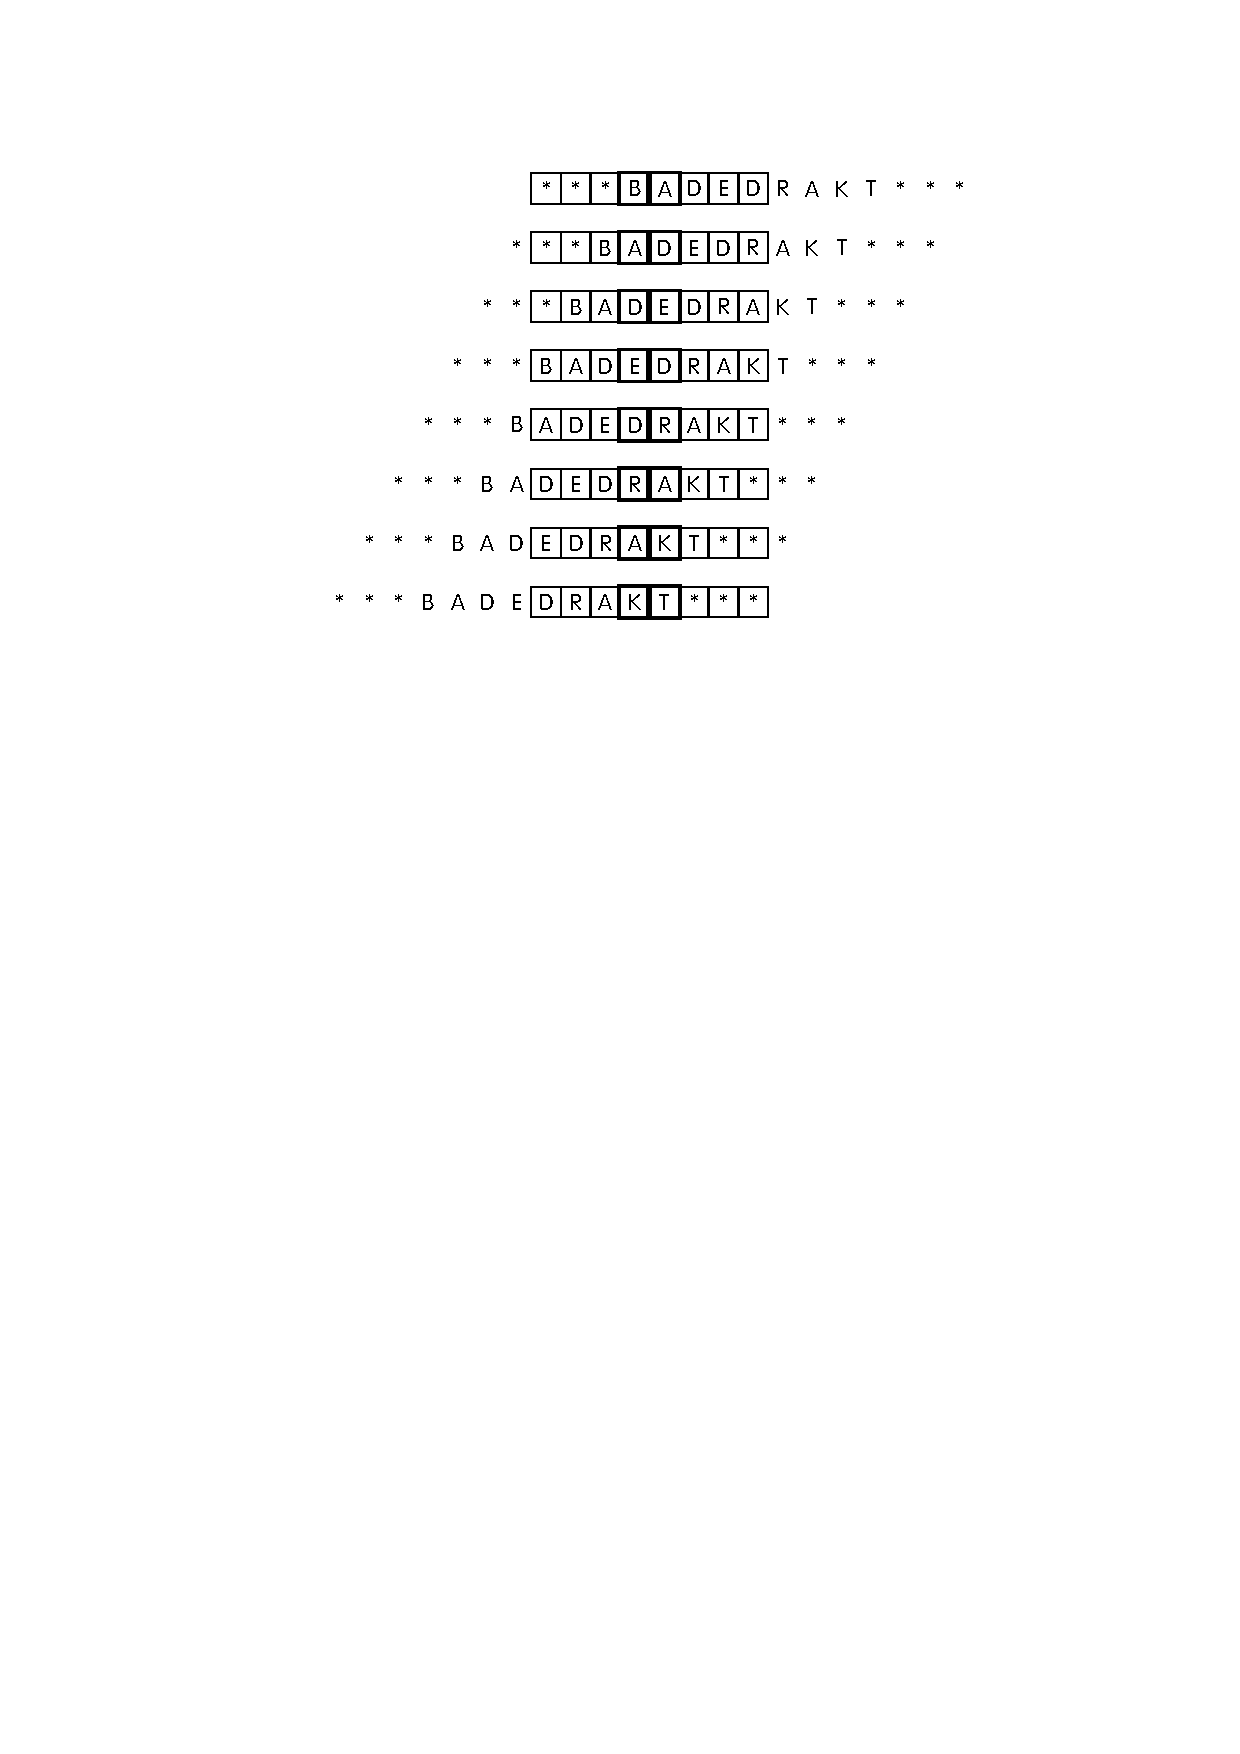
\includegraphics[width=0.75\textwidth]{content/figures/vindu.pdf}
  \caption[Vindu for orddeling med nevrale nettverk]{Vindu som viser hvordan nettverket tester et ord for hvor delepunkter skal settes inn. Illustrasjon hentet fra \textit{Two approaches to hyphenating norwegian} \cite{kristensen1998two}.}
  \label{fig:vindu}
\end{figure}


Når nettverket er tilstrekkelig opplært kan vi presentere nye ord for nettverket og det vil kunne svare om det sannynligvis er ønsket med et delepunkt. Jo større vindu og større nettverk man velger jo mer nøyaktige svar får man, men nettverket vil også vokse i lagringsstørrelse. Det vil nærme seg et oppslagsverk. Riktig vindusstørrelse og størrelse på nettverket må velges for å oppnå den beste oppveingen. 

%\subsubsection{Back-propagation}
%
%[TODO: Husk å forklare hvor dette kommer fra, kanskje hente fra AI-bok]
%
%Prosesseringselementene (nodene?) i et back-propagation-nettverk organiseres i lag, der nevronene i ett lag mottar signaler direkte fra laget under og sender signaler videre til laget direkte over. Det er ikke tillatt med koblinger innad i samme lag, bortsett fra input-laget. Inputverdien til en node $j$ regnes ut fra
%
%\begin{equation}
%S_j = \sum w_{ji}a_i
%\end{equation}
%
%hvor $w(j_i)$ er vekten mellom $j$ til $i$ og $a_i$ er output fra node $i$ i forrige lag. Utverdien fra en node er
%
%\begin{equation}
%a_j = f(S_{j})
%\end{equation}
%
%hvor $f(x)$ typisk er sigmoidalfunksjonen
%
%\begin{equation}
%S(t) = \frac{1}{1+e^{-t}}.
%\end{equation}
%
%\subsubsection{Læringsfasen}
%
%Ved første oppstart vil koblingene i nettverket få utdelt tilfeldige vekter. For å lære opp nettverket mates så inn patterns (mønstere) og vektene justeres deretter. Dette foregår ved at en definerer en input (pattern) og en ønsket output (target). Så kjører man input gjennom nettverket, ser på hva som faktisk kommer ut av resultat (output), sammenligner output med target, beregner feil og justerer vektene deretter. Det man ønsker å oppnå er et sett med vekter så nettverket tilfredsstiller alle input og output-par. Feilen i nettverket (dissonansen mellom ønsket output (target -- $t$) og faktisk output (output -- $a$)) regnes ut ved:
%
%\begin{equation}
%E = \frac{1}{N}\frac{1}{2}\sum\limits_{p}\sum\limits_{i}(t_{pi}-a_{pi})^2
%\end{equation}

\subsubsection{Orddeling via nevrale nettverk}

Kristensen og Langmyhr \cite{kristensen1998two} presenterer en metode for orddelingsproblemet ved nevrale nettverk. Problemet formuleres som et ja/nei-spørsmål om det er lovlig å putte inn et delepunkt mellom to bokstaver i et ord. Ved et ord på $n$ bokstaver får $n-1$ slike spørsmål å svare på. Nettverket får ikke se hele ordet av gangen, men et vindu av en gitt lengde med bokstaver hvor ordet ruller forbi. Tomme felter i vinduet representeres med asteriks-tegnet «*». Størrelsen på vinduet kan endres, men generelt har man at større vindu vil generere mindre konflikter og mer nøyaktige resulateter, men resultere i lengere treningstid og større minnebruk. 

Hver bokstav representeres av ett nevron (altså tjueni for norsk) og ett for asterisk-tegnet. Hvert tegn vil derfor ha en lik lengde på 30 bit. Størrelsen på output-laget vil kun være ett nevron (ja eller nei), mens input-laget vil være $V$ (størrelse på vinduet) multiplisert med $\beta$ (størrelse på alfabet). Kristensen og Langmyhr velger et vindu på 8 og antall nevroner i første lag blir da, $8\times 30 = 240$. Om vi får delepunkt i midten av vinduet, mellom de to gitte bokstavene, avgjøres om aktiviteten av output-nevronet er større en grenseverdien $0,5$. 

Treningsdataen i dette eksemplet vil bestå av ni linjer, åtte til hver bokstav i vinduet og siste til output-refereanseverdi. Eksempelvis, har vi treningsmønsteret \texttt{***|SE|KVE}, som spesifiserer at det er uønsket med delepunkt mellom \texttt{S} og \texttt{E}, representeres det på måten illustrert i figur~\ref{fig:ordmonst}. I kapittel~\ref{sec:dag-tex}, som tar for seg tidligere areid, viser resultater fra denne fremgangsmåten.

\begin{figure}
\begin{verbatim}
000000000000000000000000000001
000000000000000000000000000001
000000000000000000000000000001
000000000000000001000000000000
000001000000000000000000000000
000000000001000000000000000000
000000000000000000001000000000
000001000000000000000000000000
0
\end{verbatim}
\caption[Eksempel på treningsmønster for nevrale nettverk]{Eksempel på treningsmønster for sekvensen \texttt{***|SE|KVE}.}
\label{fig:ordmonst}
\end{figure}


\section{Regelbaserte metoder}

De regelbaserte orddelingsalgoritmene tar grunnlag i de offisielle orddelingsreglene for et gitt språk, og prøver så godt det lar seg gjøre å klassifisere ord inn i grupper og påføre de gjeldene reglene.

Los Angeles Times utviklet en regelbasert orddelingsalgoritme som skulle brukes i deres system for tekstsetting. Algoritmen registrerte og klassifiserte ord inn i vokal- og konsonantmønstere, som igjen ble delt inn i fire forskjellige grupper hvor de gjeldene reglene ble påført. I tilegg la de til regler for spesielle tilfeller og regler for håndtering av prefiks- og suffiksregler. Denne tilnærmingen ble beskrevet til å være 85--95 prosent nøyaktig. \cite{liang1983word} De nevner her ikke hvor mange feiltreff denne algoritmen generelt sett har. 

Slike tilnærminger kan ha flere svakheter. Først av alt er det en svært lite generell tilnærming til problemet. Forskjellige språk kan ha svært forskjellige regler for orddeling, og algoritmene må enten drastisk tilpasses eller skrives helt på nytt for å kunne benyttes med et annet språk. En slik tilnærming er også problematisk for språk hvor delepunktet er basert på uttale av ordet, slik som amerikansk-engelsk. Uttale kan raskt endre seg over tid, og da er man nødt til å endre selve algoritmen for å omfavne disse nye endringene. Det holder ikke å endre noen parametere, eller kjøre et program med ny inputdata for å tilpasse resultatet, slik det kan være mulig med de andre tilnærmingene. Et annet problem er at det alltids finnes unntak fra regler og en liste som utfyllende skal beskrive alle unntak kan bli unødvendig stor og vanskelig å håndtere. Til sist, sammensatte ord, som vi har mye av i det norske språket, kan være vanskelig for en datamaskin å analysere korrekt. Hvordan skal en datamaskin kunne forstå at «fylkestrafikksikkerhetsutvalgssekritariatslederfunksjonene» er en sammensatt kombinasjon av mange ord og at den må finne alle disse sammensettningene for å finne riktig delepunkt? For ikke å nevne at den også må gjennkjenne komposisjonsfuger i ordet. \cite{liang1983word,thoresen1993virtuelle}